\documentclass[english,a4paper,12pt,reprint]{revtex4-1}
\usepackage[T1]{fontenc} %for å bruke æøå
\usepackage[utf8]{inputenc}
\usepackage{graphicx} %for å inkludere grafikk
\usepackage{url}
\usepackage{physics}

\usepackage{multirow}
\usepackage[english]{babel}
\usepackage{verbatim} %for å inkludere filer med tegn LaTeX ikke liker
\usepackage{mathpazo}
\usepackage{amsmath}
\usepackage{listings}
\usepackage{varioref}
\usepackage{booktabs}

\usepackage{cleveref}
\usepackage{bm}

\usepackage{siunitx}
\usepackage{gensymb}
% \usepackage{mhchem}
\usepackage{textcomp}

% \usepackage{lettrine}
% \usepackage{calligra}
% \renewcommand{\lettrineFontHook}

\newcommand*\diff{\mathop{}\!\mathrm{d}}

\setcounter{tocdepth}{2}
\newcommand{\rmd}{{\mathrm d}}

\newcommand{\oder}[2]{\frac{{\rm d}#1}{{\rm d}#2}}
\newcommand{\od}[1]{\frac{{\rm d}}{{\rm d}#1}}
\newcommand{\odder}[2]{\frac{{\rm d}#1}{{\rm d}#2}}
\newcommand{\pd}[1]{\frac{\partial}{\partial #1}}
\newcommand{\pdt}[2]{\frac{\partial #1}{\partial #2}}
\newcommand{\pddt}[2]{\frac{\partial^2 #1}{\partial #2^2}}
\newcommand{\tpddt}[2]{\tfrac{\partial^2 #1}{\partial #2^2}}
\newcommand{\pdtfix}[3]{\frac{\partial #1}{\partial #2}_#3}

\newcommand{\spdt}[2]{\partial #1/\partial #2}
\newcommand{\npdt}[3]{\frac{\partial^{#3} #1}{\partial #2^{#3}}}

\newcommand{\angstrom}{\mbox{\normalfont\AA}}

\lstset{language=Matlab,                        % Use MATLAB
        frame=single,                           % Single frame around code
        basicstyle=\small\ttfamily,             % Use small true type font
        keywordstyle=[1]\color{Blue}\bfseries,        % MATLAB functions bold and blue
        keywordstyle=[2]\color{Purple},         % MATLAB function arguments purple
        keywordstyle=[3]\color{Blue}\underbar,  % User functions underlined and blue
        identifierstyle=,                       % Nothing special about identifiers
                                                % Comments small dark green courier
        commentstyle=\usefont{T1}{pcr}{m}{sl}\color{MyDarkGreen}\small,
        stringstyle=\color{Purple},             % Strings are purple
        showstringspaces=false,                 % Don't put marks in string spaces
        tabsize=5,                              % 5 spaces per tab
        %
        %%% Put standard MATLAB functions not included in the default
        %%% language here
        morekeywords={xlim,ylim,var,alpha,factorial,poissrnd,normpdf,normcdf},
        %
        %%% Put MATLAB function parameters here
        morekeywords=[2]{on, off, interp},
        %
        %%% Put user defined functions here
        morekeywords=[3]{FindESS, homework_example},
        %
        morecomment=[l][\color{Blue}]{...},     % Line continuation (...) like blue comment
        numbers=left,                           % Line numbers on left
        firstnumber=1,                          % Line numbers start with line 1
        numberstyle=\tiny\color{Blue},          % Line numbers are blue
        stepnumber=5                            % Line numbers go in steps of 5
    }


\graphicspath{{figures/}}
\bibliographystyle{plain}

% \renewcommand{\contentsname}{Innhold}

\addto\captionsnorsk{% Replace "english" with the language you use
  \renewcommand{\tocname}%
        {Innhold}%
}

\begin{document}

\title{\textsc{The LEGO Watt balance}}
\author{\textsc{Halvard Sutterud and Ivar Haugerud}\\\textsc{University of Oslo}}
\date{\today}

\begin{abstract}
In the hopes of replicating the watt balance, which will be used in the redefinition of the kilogram, a LEGO version is constructed . The study is based on the same apparatus made by NIST \cite{chao_lego_2015}. The LEGO watt balance uses both electromagnetic and mechanical power in it's weighing, with two different modes; velocity and force mode. The two modes makes the imprecise variables to measure cancel out, and a precise value for the mass of an object, and Planck's constant can be found. Our construction of the watt balance did not live up to the expectations. Both the mass and Planck's constant deviated with a factor of two compared to the correct value. The deviation has it's root in the coils used in our experiment.

\end{abstract}

\maketitle{}

\section{Introduction}
Since 1889 the kilogram has been defined by the mass of an object, called the IPK, \textit{international prototype kilogram}. The IPK was forged in 1879, and is made of $90\%$ platinum and $10\%$ iridium. The kilogram is the only base SI unit which is still defined by a physical object, but this will change this year, 2018, where the kilogram will be defined by a watt balance through a fixed value of Planck's constant. A reason for the proposed change in the definition of the kilogram, is to make the kilogram more presice, and more universal. There exists many copies of the IPK around the world. When calibrating these \textit{identical} copies it has been measured a drift in mass, \vref{drift_kg}. At $\Delta m = 0$ is the IPK, which has zero uncertenty in it's mass, and relative to this the drift of it's sisters. Even though all of the IPK's has been stored carefully, it has been measured a change in mass of over $\SI{50}{\micro\gram}$ since 1889. Due to this, the IPK has most likely changed it's mass as well. A redefinition of the kilogram would remove this problem, as well as making one of the most import base SI units more precise. The redefinition would also make physics more universal, since the precise measurement of mass would no longer relay on a calibration from a weight in Paris. The previous redefinition of an SI units was done in 1960 by defining the meter to the wavelength of light from a specific source. It is now time to put the 129 year old definition of the kilogram to rest, and make the last base SI unit derivable from physical phenomena.\\
The experiment in this report is carried out in the hopes of replicating the redefinition of the kilogram which will take place in 2018. This will be done by constructing a less precise version of the watt balance. Our construction is based on a LEGO watt balance designed by the national institute for standards in technology, NIST \cite{chao_lego_2015} and A. Geelmuyden and S.G. Winther-Larsen's \cite{August} construction. Instead of using a multiple of Planck's constant from the Josephson effect, we will use a standard electrical circuit, a shadow sensor, two lasers, and LEGO to construct the weight. This will be done by using the Lorentz' force from electromagnetism, to create a mechanical, and electromagnetic, power which will gives us an expression for the mass of the object. This method will cancel out the variables which are hard to measure precisely in the expression for the mass, and we will be left with four variables which we can measure precisely using the LEGO watt balance.

\begin{figure}
  \centering
  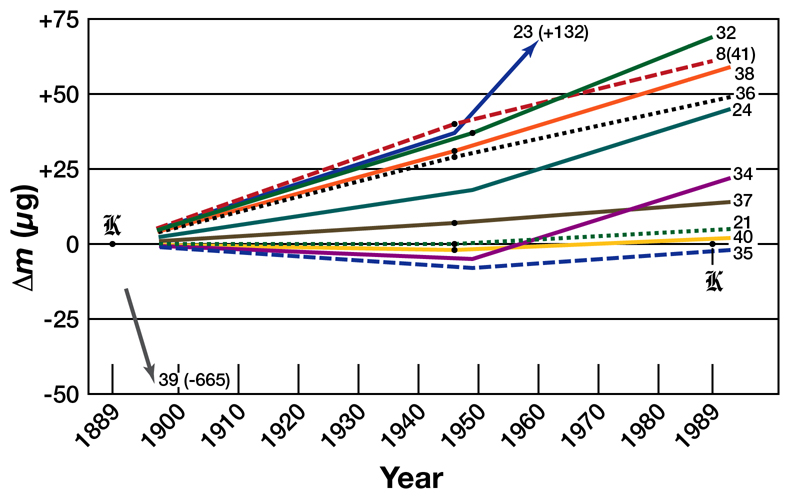
\includegraphics[scale=0.305]{Prototype_mass_drifts.jpg}
  \caption{The drift over time of the IPK's sister copies is shown. At $\Delta m$ = 0 we see the IPK, which is by definition equal to the kilogram. The drift in mass of the IPK's copies tells us that the kilogram is changing over time, and that a redifinition is needed.}
  \label{drift_kg}
\end{figure}

\section{Theory}
The LEGO watt balance has it's name from combining mechanical power and electrical power, both with the unit watt, and solving the equation for the mass $m$ in kilogram. Acquiring the mechanical power and the electrical power is done by having the Kibble balance in two different modes, velocity mode and force mode.


\subsection{Velocity mode}
From Maxwell's equations one can derive that the magnetic flux through a coil is
\begin{equation}
\Phi = \int\int_A \bm{B} \cdot \diff \bm{A},
\end{equation}
where we take the dot product between the magnetic flux density vector $\bm{B}$ with the  normal vector of the infinitesimal cross section $\diff A$, and sum over this in an integral. Faraday's law of induction states that a change in magnetic flux, induces an electrical potential $V$ over the coil

\begin{equation}
    V = N\frac{\diff\Phi}{\diff t}, \label{induced_volt}
\end{equation}

where $N$ is the number of windings in the coil and $\diff\Phi/\diff t$ is the change of the magnetic fluc through the coil over time. If the direction of the magnetic flux density is equal to the normal vector of the cross section, and the infinitesimal area vector can be written as $l\diff \bm{z}$ where $l$ is the circumference of one winding of the coil, and $\diff \bm{z}$ is a small change in the height of the coil. With this we can write $\diff \Phi$ as $B\diff \bm{A} = Bl\diff z$. With this substitution we can write equation \eqref{induced_volt} as
\begin{equation}
    V = N\frac{\diff}{\diff t}\left(BL\right)_v\diff z = NlBv,
\end{equation}where we have used that the total length of the coil is the number of windings $N$ multiplied by the circumference $l$. In this expression $v$ is the velocity of the magnetic object traveling through the coil. From this we can write the induced voltage as
\begin{equation}
    V = \left(BL\right)_vv. \label{voltage}
\end{equation}
By finding the slope of the best straight line between voltage and velocity, we can obtain the value of $\left(BL\right)_v$.

\subsection{Force mode}
A regular equal-arm balance relays on comparing a calibrated mass with an unknown mass. Instead of using a know mass, we will use a force induced from the Lorent'z force by
\begin{equation}
    \bm{F} = I\int_c \diff \bm{l}\cross B, \label{lorentz_force1}
\end{equation}
where $I$ is the current through the coil, and $\bm{B}$ is the magnetic flux density, and we integrate over infinitesimal lengths of the coil $\diff \bm{l}$. The magnetic flux density will be tangential to the change of the coil, and cross product of these two will result in the force working in the $z$-direction. The magnitude of this force will be the integral of $\diff l$ along the coil, which result in
\begin{equation} \label{force_mode_force}
    F_z = \left(BL\right)_FI.
\end{equation}
This force will cancel out the gravitational force due to gravity $g$ on an object with mass $m$, such that
\begin{equation}
    \left(BL\right)_FI = mg. \label{mechanical}
\end{equation}
This measurement will be done multiple times to reduce the uncertainty. We can then relate the current $I_{1,2,3}$ used to stabilize the tar mass, and the current $I_{2,4}$ to stabilize the the known mass $m$, the gravitational constant $g$ to the magnetic flux density times the length of the wire by
\begin{equation}
    I = \frac{1}{3}\left(I_1 + I_3 + I_5\right) - \frac{1}{2}\left(I_2 + I_4\right) = \frac{mg}{\left(BL\right)_F}. \label{multiple_measur}
\end{equation}

\subsection{Calculating the mass}
From the two previous sections, we have two expressions which both share the common factor $BL$. This means that we can relate the two equations to each other by substitution of $BL$
\begin{equation}
    VI = mgv.
\end{equation}
This equation relates the electromagnetic power with the  mechanical power. By doing this we remove the two measurements of the experiments which is the hardest to measure precisely, and would result in the largest uncertainties. This equation can easily be solved for the mass $m$
\begin{equation}
    m = \frac{VI}{gv}.\label{mass}
\end{equation}
\\

\subsection{Measuring Planck's constant}
Due to how the present unit system is structured it is possible to measure Planck's constant with the LEGO watt balance. Since 1990 almost all electrical calibration has done by a different unit system than the SI-system, the conventional units. The conventional units used the Josephson ($K_{j-90}$) and von Klitzing constants ($R_{K–90}$) as fixed values. With the LEGO watt balance we can relate the mechanical power in SI units, to the electrical power in conventional units
\begin{equation*}
    \{VI\}_{90} = \{mgv\}_{SI},
\end{equation*}
where the indices denote the unit for the conventional value, $90$, or SI units, SI. The ratio between watt in the SI units and watt in the conventional units is
\begin{equation}
    \frac{\{mgv\}_{SI}}{ \{VI\}_{90}} = \frac{\text{W}_{90}}{\text{W}_{SI}} = \frac{h_{SI}}{h_{90}} \label{relate_units}.
\end{equation}
Where $h_{90}$ is Planck's constant in conventional units, defined as \begin{equation}
    h_{90} = \frac{4}{K_{j-90}\,R_{K–90}} = 6.626068\ldots\text{Js}.
\end{equation}
Equation \eqref{relate_units} can be solved for Planck's constant $h$ in SI units
\begin{equation}
    h = h_{90}\frac{\{mgv\}_{SI}}{ \{VI\}_{90}}. \label{planck}
\end{equation}


\section{Experimental}
\subsubsection*{\textsc{List of parts}}
\begin{itemize}
  \item Multimeter (Fluke 45)
  \item Laser (Line laser module LN60-650)
  \item Shadow sensor  (Mouser electronics first sensor PC50-7-TO8)
  \item Data acquisition box (2 $\times$ National Instruments USB6211)
  \item Laser distance measure (Bosch PLR30 C)
  \item Linear voltage regulator (ON semiconductor LM317)
  \item Weight  (Pro scale XC 500)
  \item Voltage generator (Delta Elektronika SM 3004-D)

\end{itemize}
\subsection{\textsc{System}}
An illustration of the watt balance is shown in \cref{fig:watt_balance}, where the most important parts are highlighted and given a reference letter. They include the two magnets, the two coils, both lasers and the shadow sensor. Most of the weight except from these parts and the wires were made from LEGO. The lever is not connected to the main LEGO structure, but rests on a smooth LEGO surface with two LEGO knives. The diameter of the LEGO knives are $\SI{0.72}{\milli\meter}$. This lets the lever with connected mass pans and magnets oscillate freely while the structure and coils stand still.

\begin{figure}
  \centering
  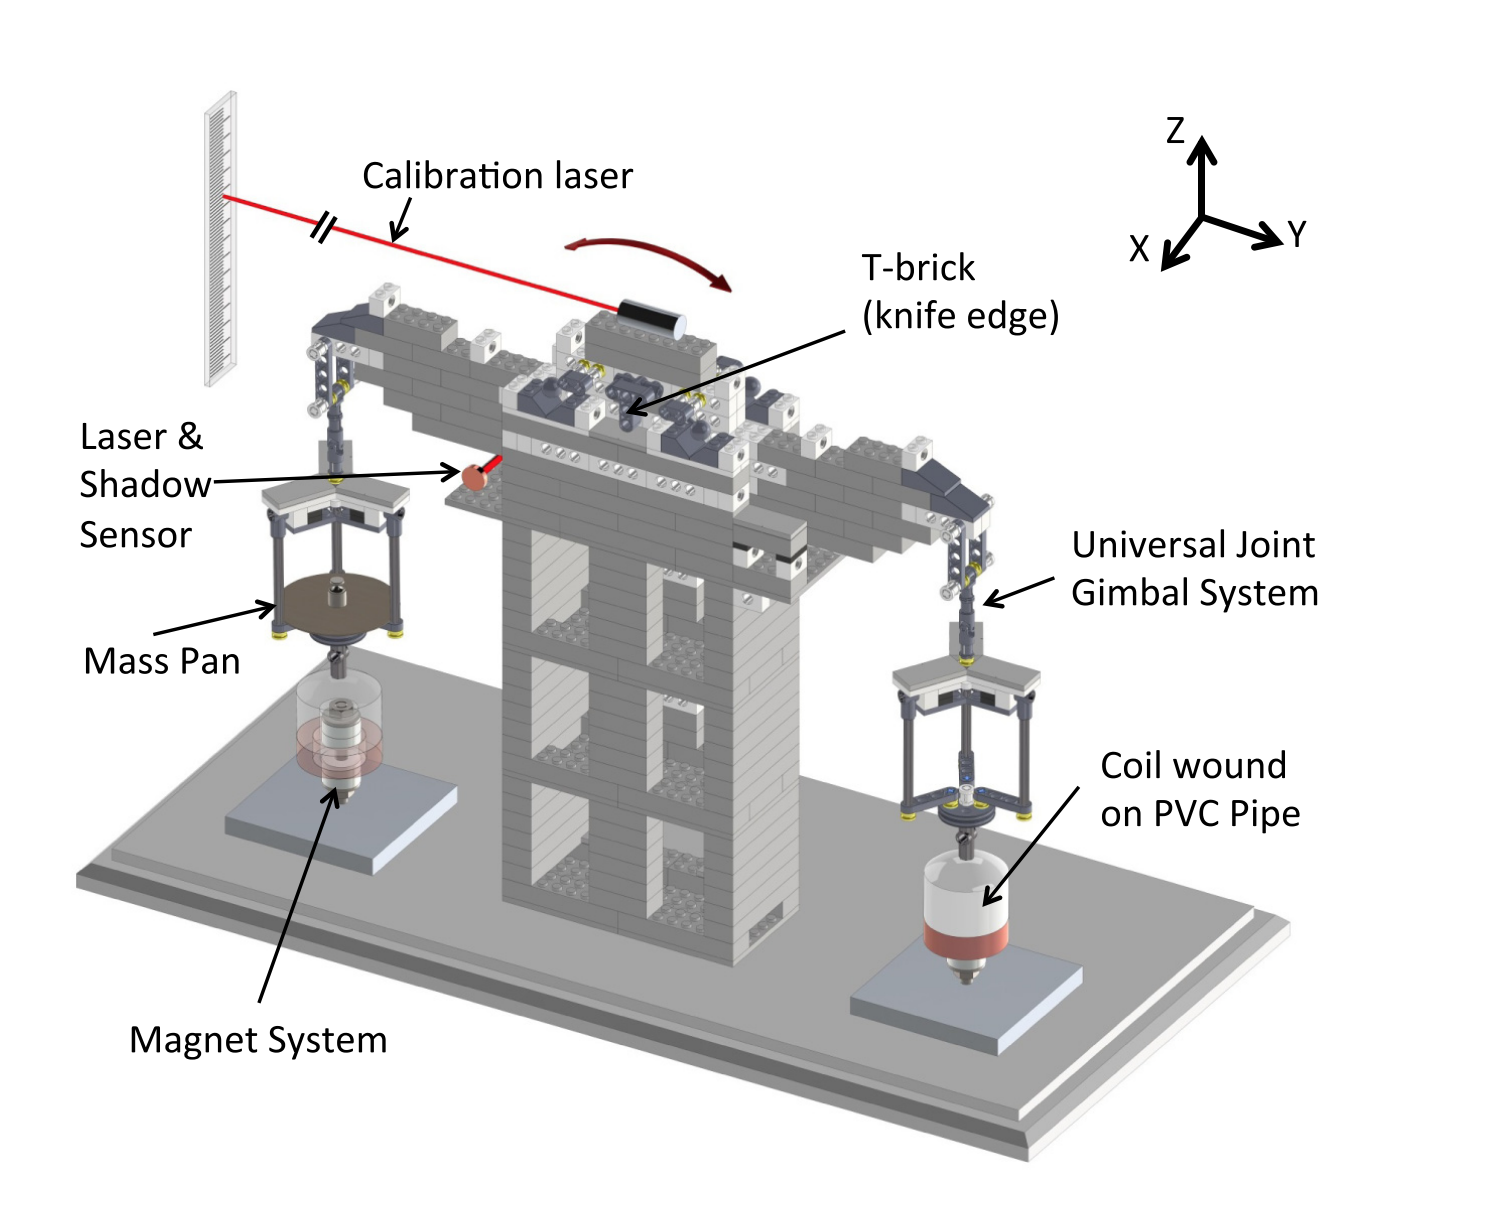
\includegraphics[scale=0.37]{LEGO_watt_fig.png}
  \caption{Illustration of the LEGO watt balance. The important parts of the experimental setup is shown clearly with name.}
  \label{fig:watt_balance}
\end{figure}



\subsubsection{\textsc{Coils and magnets}}
\begin{figure*}
  \centering
  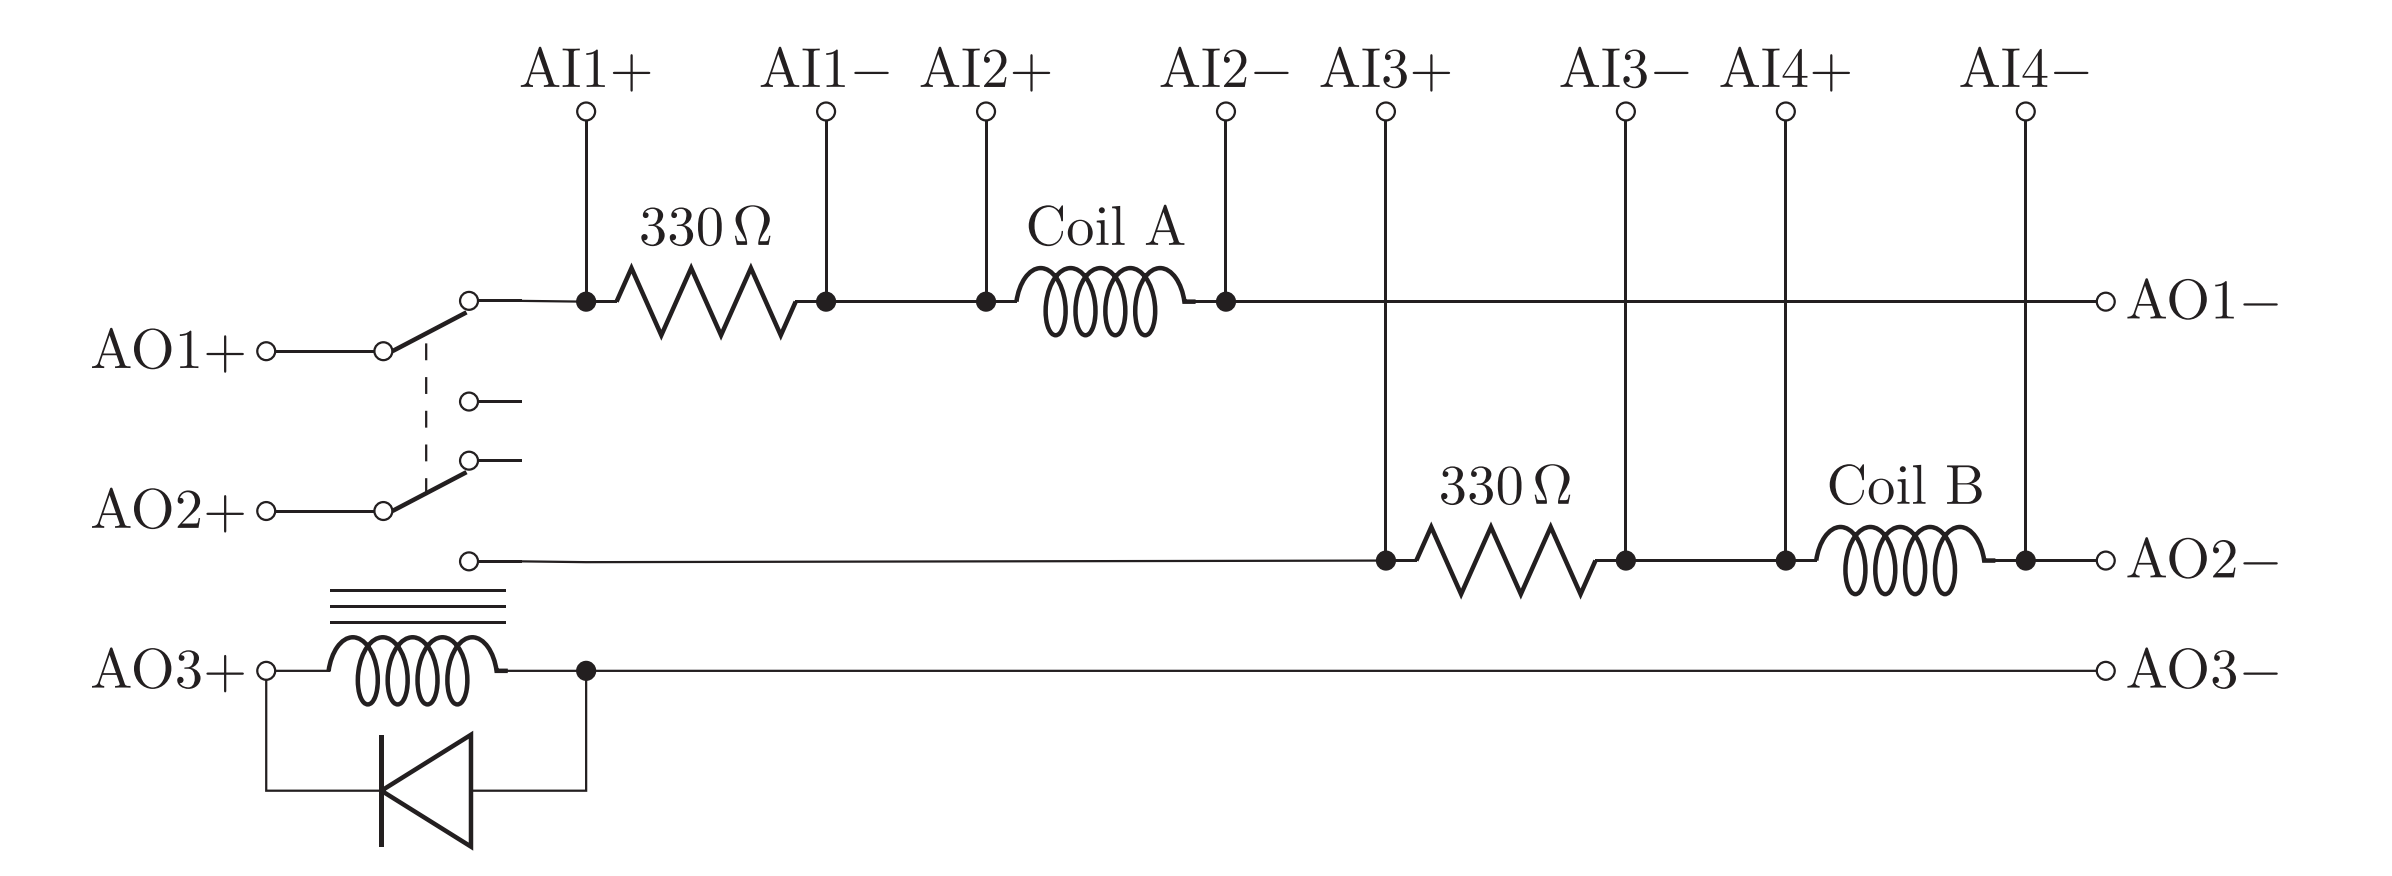
\includegraphics[scale=0.30]{coil_circuit.png}
  \caption{Circuit diagram for the coil $A$ and $B$. This diagram shows the setup for both measurements and driving of the two coils.  }
  \label{fig:coil_circuit}
\end{figure*}
The coils were made of plastic and had around $10 000$ windings of $0.1$mm copper wire over $6$cm. The coils had an inner diameter of $2.6$cm to not hinder the magnets movement, but still keep the distance to the windings small. When choosing the coil there is a trade off between high inductance and high resistance. More windings gives a higher inductance, but increases the resistance. For the coils used in this experiment we need a high inductance, and then had to settle for a high resistance, measured to be $\SI{335}{\ohm}$. As we can see in \vref{fig:watt_balance} we use two identical coils, one for each magnet. The two different coils, $A$, and $B$, have different purposes. Coil $A$ is the driver coil. It will have a known, sinusoidal, current through the wires in order to force the movement of the magnets to make measurements in velocity mode. Coil $B$ on the other hand, will be used both as a reader coil in velocity mode and as the counteracting coil in force mode. The measurements from the reader coil was directed to a data acquisition box, with Matlab scripts for calibration routines and measurements. The circuit for the coils is shown in \vref{fig:coil_circuit}. \par
The neodymium magnets moving inside the coils are two identical magnets facing each other with the same pole. This makes the magnetic field point radially outwards, which is necessary for the Lorentz force \eqref{lorentz_force1} to be directed up and down.


\subsubsection{\textsc{Laser and shadow sensor}}

\begin{figure*}
  \centering
  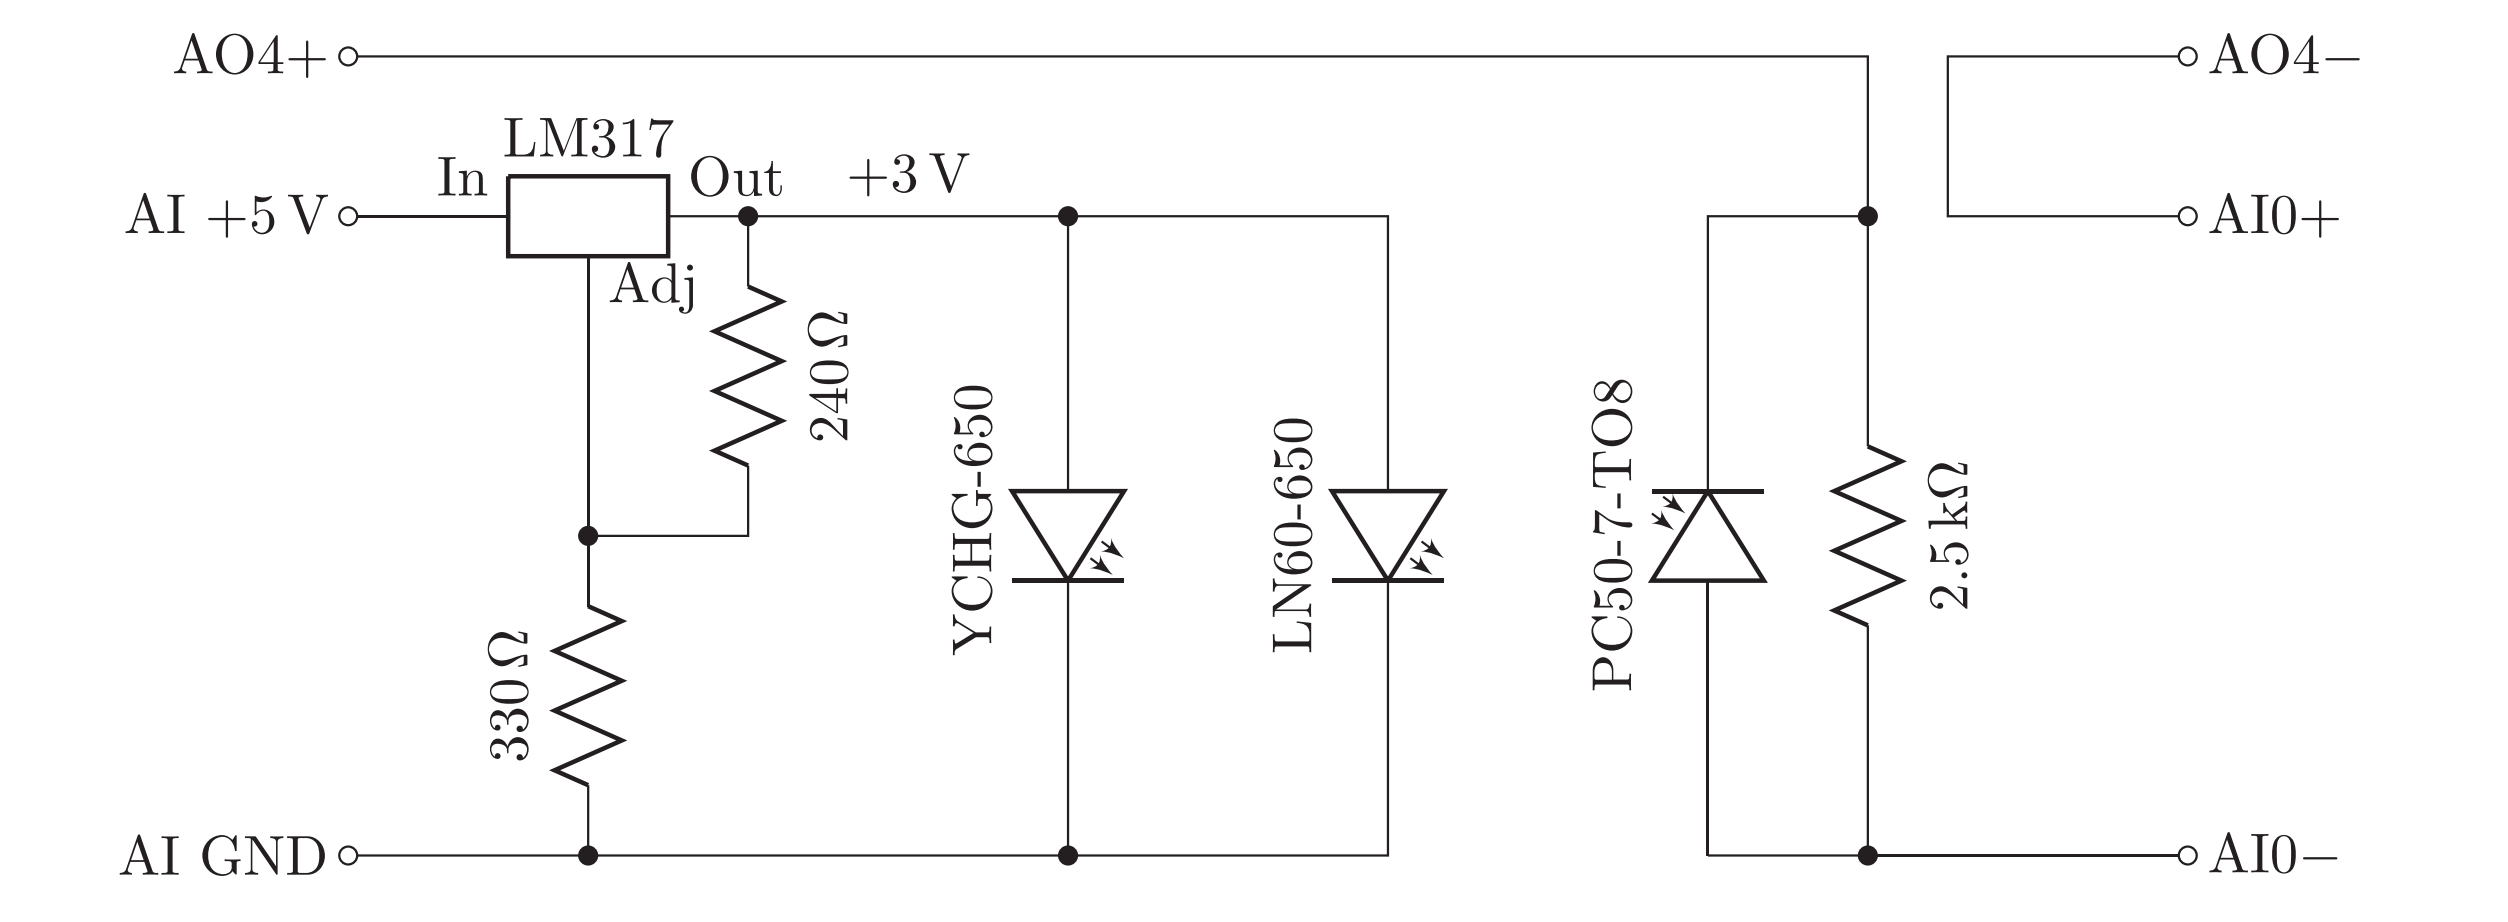
\includegraphics[scale=0.30]{laser_shadow_circuit.png}
  \caption{Circuit diagram for measuring the output of the shadow sensor, as well as giving a stable voltage to the laser.}
  \label{fig:circuit_laser}
\end{figure*}

To know the vertical position of the magnets it is sufficient to know the angle of lever. To measure this angle a laser is placed by the lever as shown in \cref{fig:watt_balance}. The laser sends out light with a wavelength of $\SI{650}{\nano\meter}$, which is registered by the shadow sensor, also shown in \cref{fig:watt_balance}. The movement of the lever will be measured by the amount of light the shadow sensor receives from the laser. The position of the laser and the shadow sensor has to be carefully placed as to not get saturated by the maximum or minimum amplitude of the lever. If this is the case the measurements a lot of information would be lost. An illustration of the laser and shadow sensor is shown in \cref{fig:shadow_sens}.

\subsubsection{\textsc{Data acquisition}}
To read the measurements from the coils and the shadow sensor we used two data acquisition boxes (DAQ). The use of the two DAQ boxes is shown in the circuits, \vref{fig:coil_circuit} and \vref{fig:circuit_laser}. Using the programming language MatLab we were able to send controlled signals to both the coil and the laser. For the laser the DAQ box delivered a constant voltage of $\SI{0.35}{\volt}$. For the driver coil the DAQ box had to deliver a sinusoidal voltage with the same frequency in resonance with the system. The DAQ box made it possible to analyse the data during the experiment, as well as easily controlling the voltages over the circuit.

\subsection{Calibrating shadow sensor}
To find the relationship between the amount of light received from the shadow sensor and the angle of the lever, a laser was placed on top of the lever. The laser was directed towards a wall, at a known, long distance, away from the rotational axis of the lever. By having the lever stationary at a certain angle and measuring the output from the shadow sensor and the position of the laser relative to the equilibrium position, we can measure the relationship between the output of the shadow sensor and the angle of the lever. The electrical circuit to measure the output of the shadow sensor, and drive the laser, is shown in \vref{fig:circuit_laser}.

\begin{figure}[h!]
  \centering
  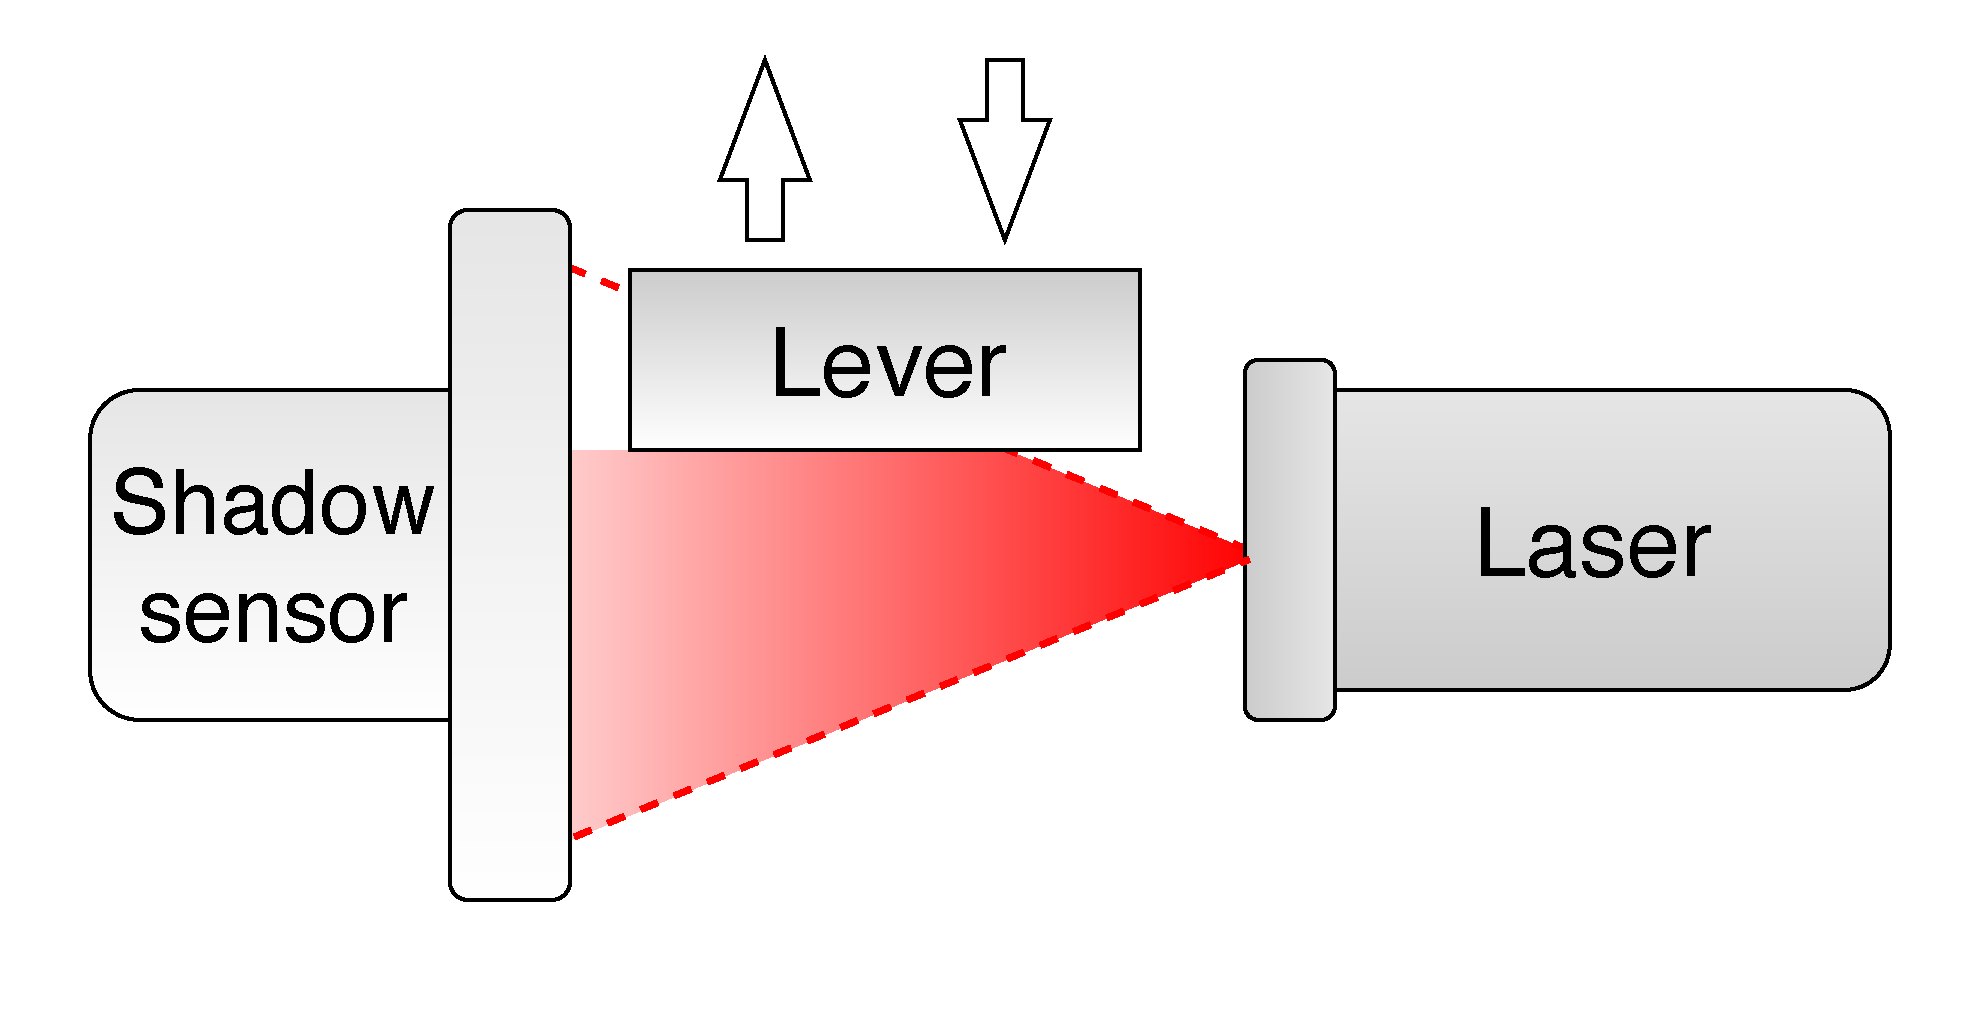
\includegraphics[scale=0.21]{shadow_sensor.pdf}
  \caption{Illustration of how the shadow sensor and laser is used to measure the angle of the lever. This figure also illustrates the problem of saturating the shadow sensor with too large amplitude of the lever.}
  \label{fig:shadow_sens}
\end{figure}

\subsection{Velocity mode}
The calibration of the shadow sensor gives us the relationship between the output of the shadow sensor, and the angle of the arm. By measuring the length from the pivot point to the magnets we can find the $z$-component of the position of the magnets from reading the output from the shadow sensor. By derivating this position with respect to time, we can find the velocity of the magnets. \\
For the system to be set in motion a sinusoidal current is passing through the driving coil. The frequency of the sinusoidal signal is found by taking using Fourier transform on the movement of the arm, to find the resonance frequency of the system, and choosing this as the signal frequency. When this frequency is found, we choose an amplitude which where the movement of the arm does not saturate the shadow sensor. To measure $\left(BL\right)_v$ the least squares method is used to find the best fit linear equation between the voltage induced in the reader coil against the velocity calculated by the numerical derivative from the shadow sensor. The slope of the straight line is then calculated to obtain  $\left(BL\right)_v$ with equation \eqref{voltage}.



\subsection{Force mode}
In force mode the driving coil is used to apply a constant force to one of the magnets. This force will neglect the gravitational force acting on an object on the other arm of the lever. To make the electromagnetic force cancel out the mechanical force we measure the output of the shadow sensor as we change the magnitude of the voltage difference over the driving coil. The magnitude can be changed until the output of the shadow sensor is equal to the output at equilibrium without the forces. To change the output voltage we use a voltage generator. This processes can be automated using a PID-control, but for this part of the experiment we chose the more practical option.
This measurements has to be done in several steps. We start with no weight on either arm, and the system in equilibrium. A tare mass $m_\tau$ is placed on one of the mass pans. This takes the system out of the null-position, and a current $I$ is applied to cancel the gravitational force due to the mass \eqref{force_mode_force}. \\
Then a secondary mass $m$ is placed on the opposite arm, and a new current $I_2$ is found to put the system in it's null position. This is done multiple times to control any drift in the measurements. When one is satisfied equation \eqref{multiple_measur} is used to relate the current, the known mass and the gravitational constant to the magnetic field times the length of the wire in force mode $(BL)_F$.\\
This is the last piece needed, and we are now able to find the mass $m$ using equation \eqref{mass}.


\section{Results}
\subsection{Calibrating shadow sensor}
To calibrate the shadow sensor we measured the voltage output from the shadow sensor while measuring the laser position against a wall. By knowing the distance from the rotational axis to the wall, and measuring the change in the position of the laser, we found a linear relationship between the position of the laser and the output of the shadow sensor. The measurements are shown in \vref{fig:result_shadow_sens}. By using the least squares method we find that the best fit line has a constant term of $c = \SI{0.8\pm0.1}{\centi\meter}$, and a slope of $m = \SI{0.337\pm0.004}{\centi\meter/\milli\volt}$. The distance from the rotational axis to the wall/c was measured with a laser distance measurer to be $\SI{0.0}{\meter}$.

\begin{figure}[htpb]
  \centering
  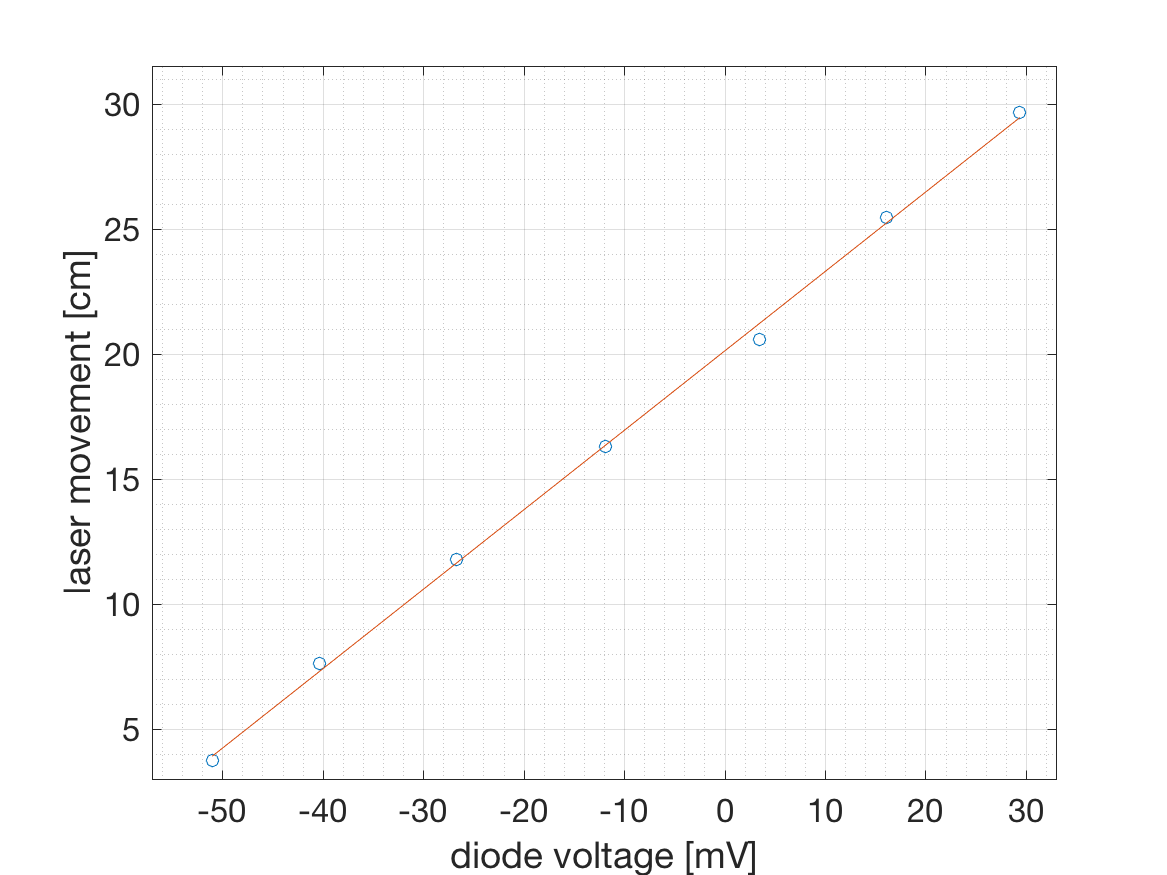
\includegraphics[scale=0.45]{laser_data.png}
  \caption{Measurements of the position of laser versus voltage output of shadow sensor. The linear relationship between voltage and position is clear.}
  \label{fig:result_shadow_sens}
\end{figure}

\subsection{Velocity mode}

The resonance frequency of the system was set equal to $\SI{0.48}{\hertz}$, and an amplitude of $\SI{0.2}{\volt}$ was used to create the oscillations. The phase space of velocity mode measurement can be seen in \cref{fig:phase_space}, where position and velocity is represented by the voltages output from the light sensitive diode and the reader coil respectively.
\begin{figure}[htpb]
    \centering
    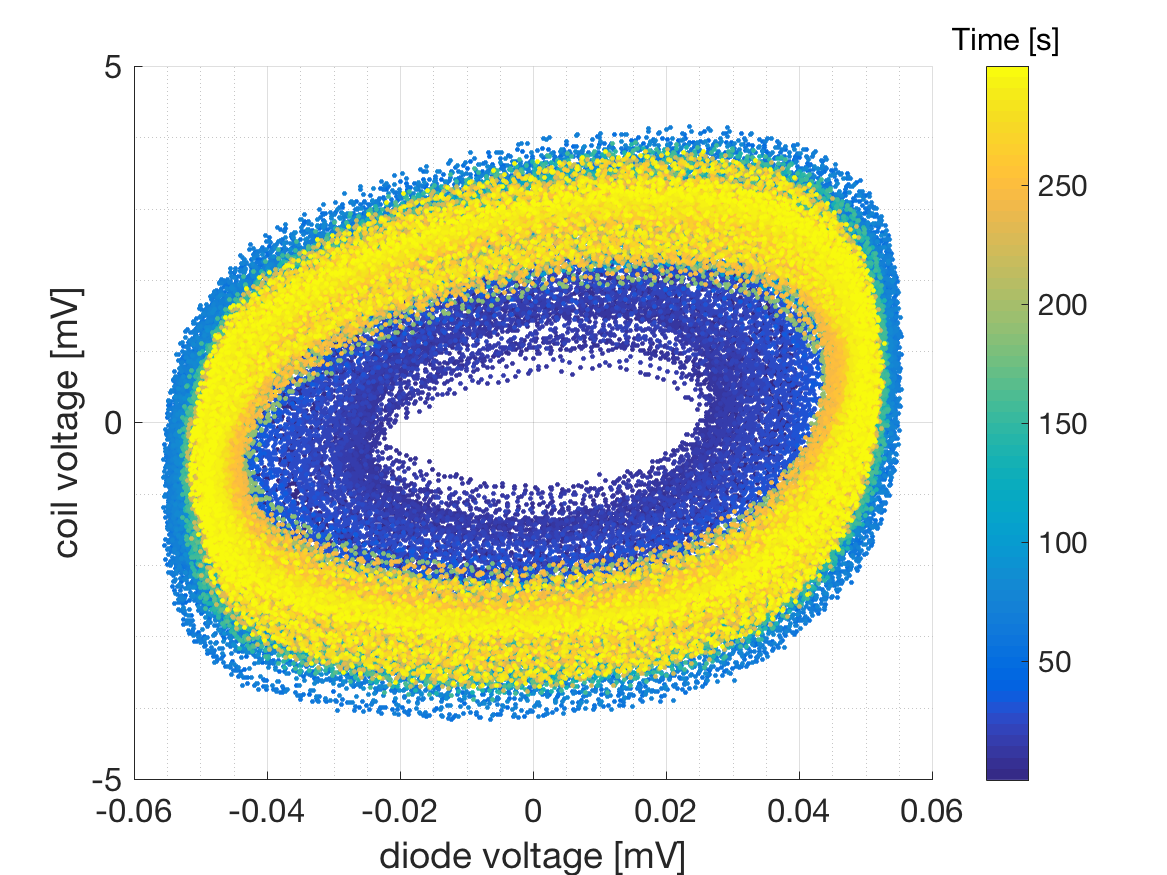
\includegraphics[scale=0.44]{phasespace.png}
    \caption{Diode voltage versus induced coil voltage, with a frequency of $\SI{0.48}{\hertz}$ and amplitude of $\SI{0.2}{\volt}$ volt on the driver coil over $200$ seconds.}
    \label{fig:phase_space}
\end{figure}
The velocity of the magnets can be calculated by using the relationship between the output from the shadow sensor with the movement of the laser on the wall, \vref{fig:result_shadow_sens}. Using the length of one unit of LEGO as a measurement we found that the distance to the magnets from the rotational axis was $\SI{17.5}{\centi\meter}$. With this we were then able to calculate the velocity of the magnets over time. The induced coil voltage is shown versus the velocity of the magnets in \vref{fig:vel_vs_coil}.
\begin{figure}[htpb]
    \centering
    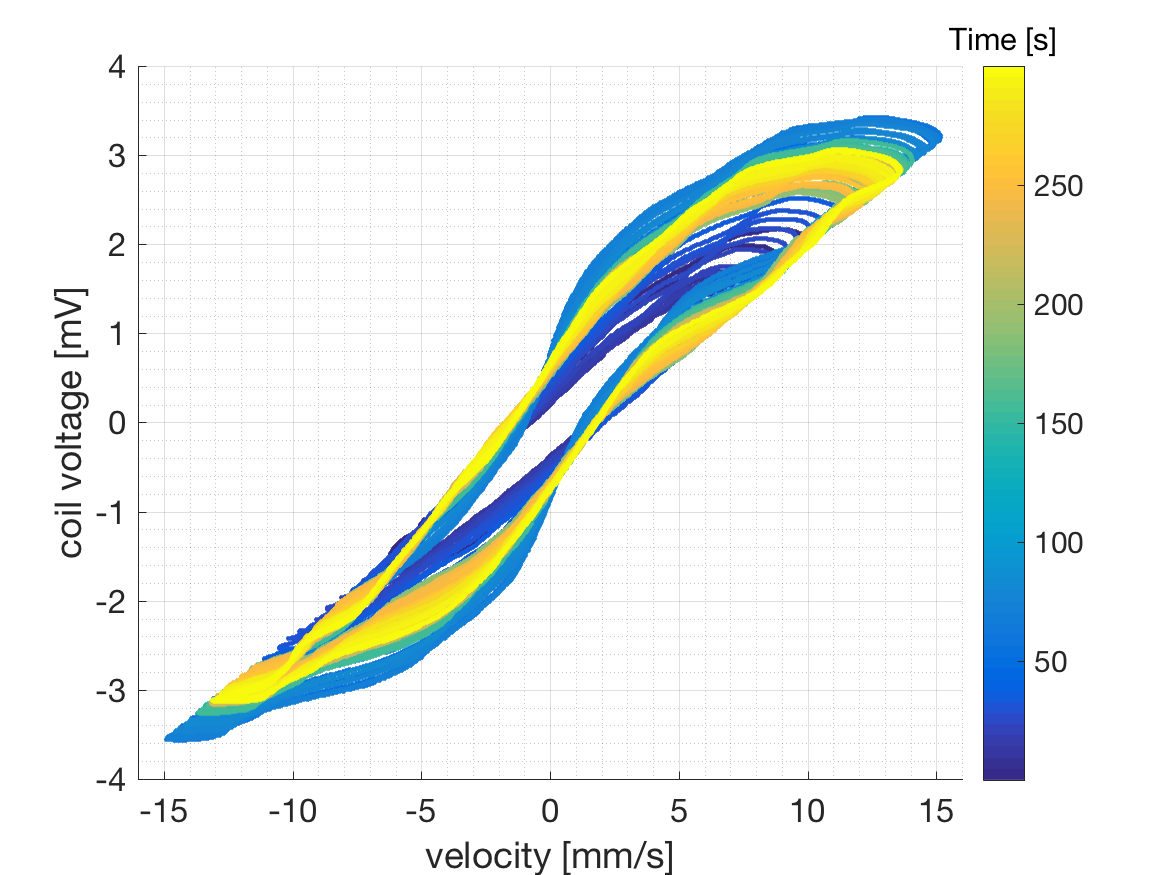
\includegraphics[scale=0.44]{vel_vs_coil.png}
    \caption{The induced voltage in the reader coil is shown versus the velocity of the magnets. This graph shows that the system is asymmetrical. The movement is different in one direction compared to the other.}
    \label{fig:vel_vs_coil}
\end{figure}
The relationship between the induced voltage, and the velocity of the magnets is linear, and the proportionality constant is $BL$ \eqref{voltage}. To obtain the value for $BL$ in velocity mode we calculate the slope in \vref{fig:vel_vs_coil} for each period. This slope is plotted versus the period number, in \vref{fig:slope}. Since the movement was dependent on the direction, \vref{fig:vel_vs_coil}, we chose to calculate the average of the slopes, for movement in one direction. We chose the slope of the bottom (TROR JEG) lines in \vref{fig:vel_vs_coil}. The value we obtain for the relationship between induced voltage $V$ and velocity $v$ is then the average of the values shown in \vref{fig:slope}. This makes the value of $\left(BL\right)_v$ be equal to $\SI{0.250\pm0.002}{\tesla/\meter}$, which we will be used to find the mass of the object we use in force mode.
\begin{figure}[htpb]
    \centering
    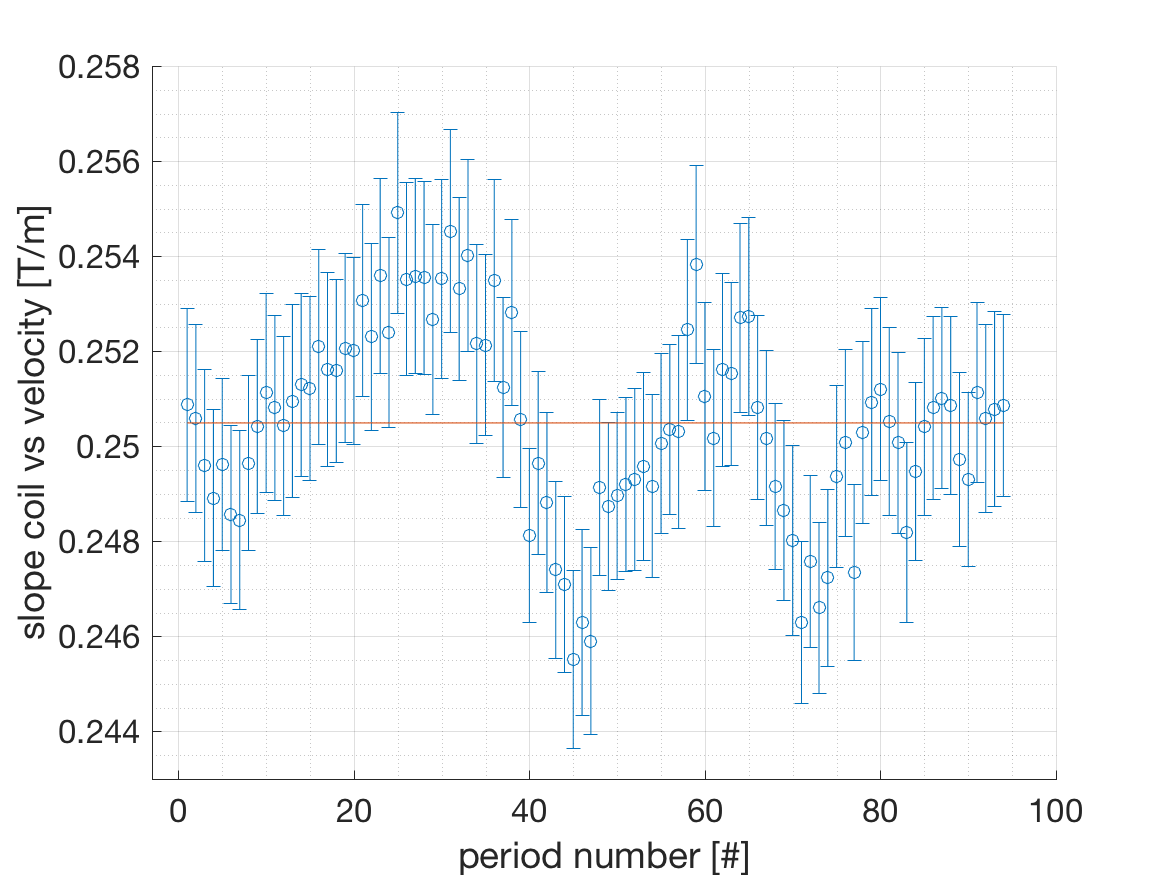
\includegraphics[scale=0.44]{slope.png}
    \caption{The slope is calculated from each period of induced coil voltage versus velocity, \vref{fig:vel_vs_coil}. From this figure we can clearly see the that the movement is asymmetrical, the slope of every even number period deviates systematically with the slope of every even numbered period.}
    \label{fig:slope}
\end{figure}

\subsection{Force mode}
We use a tare mass, $m_\tau$, and an unknown mass, $m$, and find the current required for the arm to be in equilibrium position. The measurements are shown in \vref{force_results}. From these measurements we can calculate the current $I$ using equation \eqref{multiple_measur}.

\begin{table*}
\centering
\caption{Required current to achieve equilibrium for three different masses, and the calculated value for the current used in equation \eqref{multiple_measur}. The objects used as a tare mass, $m_\tau$, and the mass we wanted to measure, $m$, was LEGO parts which where measured using a digital precision weight.}
\label{force_results}
\begin{tabular}{@{}lllll@{}}
\toprule
Weight distribution & Equalibrium current & $m_\tau = 6.73$g, $m=3.07$g & $m_\tau = 1.32$g, $m=0.67$g & $m_\tau = 1.32$g, $m=0.70$g \\ \midrule
0 - $m$  & $I_1$           & 0.1152 A                    & 0.0248 A                    & 0.0259 A                    \\
$m_\tau - m$   & $I_2$     & -0.1367 A                   & -0.0242 A                   & -0.0230 A                   \\
$0 - m$      & $I_3$        & 0.1180 A                    & 0.0248 A                   & 0.0256 A                    \\
$m_\tau - m$  & $I_4$       & -0.1351 A                   & -0.0242 A                   & -0.0232 A                   \\
$0-m$        &$I_5$       & 0.1173 A                    & 0.0245 A                    & 0.0258 A    \\ \midrule Using equation \eqref{multiple_measur} & I & 0.253 A & 0.0489 A & 0.0489 A \\ \bottomrule
\end{tabular}
\end{table*}

\subsection{Calculating the mass and Planck's constant}
Using the relationship between the induced voltage in the reader coil and the velocity of the magnets, shown in \eqref{fig:slope}, and the measurements of the current for different masses, seen in \vref{force_results}, we can calculate the mass of the object using equation \eqref{mass}. The value we use for the gravitational acceleration is $\SI{9.819}{\meter/\second^2}$. The value of the current used depends on the mass, and can be found in \vref{force_results}, the value of $V/v$ is the same for all measurements, $\SI{0.250\pm0.002}{\tesla/\meter}$. These values combined makes it possible to calculate the mass, as well as Planck's constant. The values calculated are shown in \vref{final_result}. %https://www.sensorsone.com/local-gravity-calculator/


\begin{table}[]
\centering
\caption{Measured mass and Planck's constant, compared to the proper values. As we can see, both values deviates with around a factor of two.}
\label{final_result}
\begin{tabular}{@{}lll@{}}
\toprule
Real mass {[}g{]} & Measured mass {[}g{]} & Planck's constant {[}\%{]} \\ \midrule
3.07              & 6.44                  & 48                                   \\
0.67              & 1.25                  & 54                                   \\
0.70              & 1.25                  & 56                                   \\ \bottomrule
\end{tabular}
\end{table}


\section{Discussion}

\subsection{Coil design}

The current design of the coils is not optimal. Though spreading the coils around a large area gives a more homogeneous field inside the coil when applying a current, it weakens the magnetic flux density. In reader mode, we instead want to maximize the number of windings where the magnetic flux density of the dipole magnets is largest, which is in the plane separating the two magnets. Instead, the design in the original NIST article \cite{chao_lego_2015} is probably better.

\section{Conclusion}
\bibliography{citations.bib}{}
\bibliographystyle{plain}
\end{document}
